\documentclass[paper=a4, fontsize=11pt]{scrartcl} % A4 paper and 11pt font size
\usepackage{graphicx}
\usepackage{subcaption}
\usepackage{fourier} % Use the Adobe Utopia font for the document
\usepackage{booktabs}
\usepackage{amsmath}
\usepackage{float}
\usepackage[document]{ragged2e}


\begin{document}


\begin{titlepage}

  \noindent
  \begin{tabular}{@{}p{\textwidth}@{}}
    \toprule[2pt]
    \midrule
    \vspace{0.2cm}
    \begin{center}
    \Huge{\textbf{
      Assignment 1
    }}
    \end{center}
    \begin{center}
      \Large{
        - Fast Trajectory Replanning -
      }
    \end{center}
    \vspace{0.2cm}\\
    \midrule
    \toprule[2pt]
  \end{tabular}
  \vspace{4 cm}
  \begin{center}
    {\large
      Report by%Insert document type (e.g., Project Report)
    }\\
    \vspace{0.2cm}
    {\Large
      William Lewental wfl22 \break 
Daniel Finlay dsf77 \break 
Nikhilesh Kashyap nk484
    }
  \end{center}
  \vfill
  \begin{center}
  Rutgers University\\
  Intro to Artificial Intelligence Spring 2018
  \end{center}
\end{titlepage}



	\section{Understanding the Methods}
		\subsection*{ A) Explain in your report why the first move of the agent for the example search problem from Figure 8 is to the east rather than the north given that the agent does not know initially which cells are blocked.}

\begin{figure}[h]
	\centering
	\begin{subfigure}[b]{0.4\linewidth}
		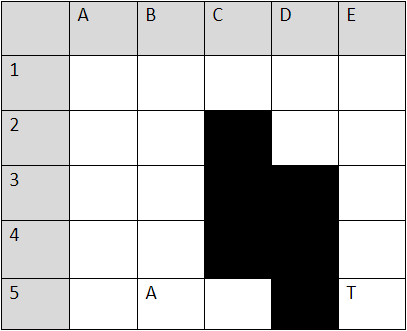
\includegraphics[width=\linewidth]{table1}
		\caption{Map}
	  \end{subfigure}
	\begin{subfigure}[b]{0.4\linewidth}
	\centering
	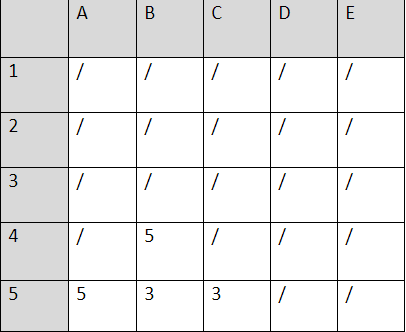
\includegraphics[width=\linewidth]{table2}
	\caption{Evaluation Function, g+h}
	\end{subfigure}
	\begin{subfigure}[b]{0.4\linewidth}
	\centering
	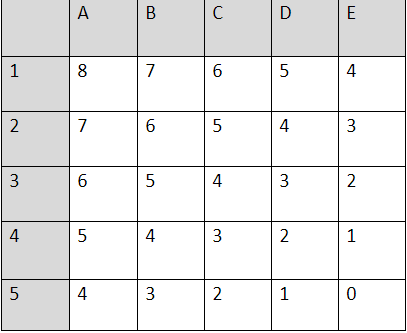
\includegraphics[width=\linewidth]{tablee3}
	\caption{Heuristic, h}
	\end{subfigure}
	\begin{subfigure}[b]{0.4\linewidth}
	\centering
	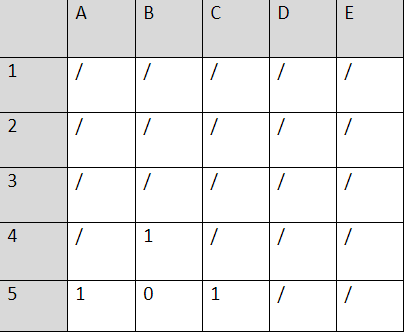
\includegraphics[width=\linewidth]{table4}
	\caption{Paid Cost, g}
	\end{subfigure}
	\caption{The Application of A*}
\end{figure}


Looking at the evaluation function for this problem, it can be seen that the first move of the agent will be to move to C5 because the evaluation function is the lowest for this block. The evaluation function is 3 for C5, while 5 for the other two blocks in the frontier set. Thus the agent will initially move to the right one space regardless that the wall is there as the agent will not be aware of the wall until the agent moves in C5.

\subsection*{ B) This project argues that the agent is guaranteed to reach the target if it is not separated from it by blocked cells.  Give a convincing argument that the agent in finite gridworlds indeed either reaches the target or discovers that this is impossible in finite time. Prove that the number of moves of the agent until it reaches the target or discovers that this is impossible is bounded from above by the number of unblocked cells squared.}

Considering that the agent is in a finite gridworld, even if the goal node is blocked, the agent will visit all of the unblocked nodes. Once all of the unblocked nodes are visited, the implementation will have an empty open list and thus the algorithm will finish. The target cannot be found and the algorithm ended in finite time. The agent will still get as close as possible to the target as the algorithm explores all cells that that have the lowest evaluation function. The most possible moves the algorithm will execute is n nodes that are unblocked. This will give us n squared maximum moves. 




\section{The Effect of Ties}
\subsection*{Implement and compare both versions of Repeated Forward A* with respect to their runtime or,
equivalently, number of expanded cells. Explain your observations in detail, that is, explain what you observed and give a reason for the observation.}

Repeated Forward A* needs to break ties to decide which cell to expand next if
several cells have the same smallest f-value.  It can either break ties in favor of cells with smaller g-values or in favor of cells with larger g-values. \newline
 When the algorithm is implemented to break ties in favor of the larger G-values, the next node selected is the node farthest from the source. This means that if the implementation is on the right path, it will reach the goal faster than if we had used the smaller G - value. However, if the implementation is not on the correct path, using the larger G-value to break ties will lead to greater deviation from the optimal path.  \newline
When the algorithm is implemented to break ties in favour of the smaller G-values, the next node selected is the node closest to the source. This implementation means that the algorithm could possibly take a greater number of steps to reach the goal then had we used the larger G- values. However, this implementation does not deviate as much from the path in the case of heading in the incorrect direction than the goal. 


\section{Forward vs. Backward}
\subsection*{Implement and compare Repeated Forward A* and Repeated Backward A*
with respect to their runtime or, equivalently, number of expanded cells. Explain your observations in detail, that is, explain what you observed and give a reason for the observation}

The difference between the runtime of Repeated Forward A* and Repeated Backward A* depends on the orientation of the blocks in the generated maps. Certain shapes lead to one method taking longing than the other to successful find the goal. In our implementation, we found Repeated Forward A* to have a faster runtime, exploring 5245.44 nodes on average while Repeated Backward A* explored 6795.66 nodes on average. 


\section{Heuristic in the Adaptive A*}
\subsection*{The project argues that "the Manhattan distances are consistent in
gridworlds in which the agent can move only in the four main compass directions." Prove that this is indeed the case.}

The Manhattan distance between two points will always be the same no matter the combination of horizontal and vertical steps. If the agent was able to move in more directions, i.e. Northwest, Northeast, the Manhattan distance would no longer be consistent because now the heuristic would overestimate the target. 

\subsection*{Furthermore, it is argued that "The h-values $h_{new} ( s )$
... are not only admissible but also consistent." Prove that Adaptive A*
leaves initially consistent h-values consistent even if action costs can increase.}

A heuristic h(n) is consistent if, for every node n and every successor n' of n generated by any action a, the estimated cost of reaching the goal from n is no greater than the step cost of getting to n' plus the estimated cost of reaching the goal from n'. This is referred to as the triangle inequality: \newline

\[h(n) \leq c(n, a, n' ) + h(n')  \]   

Following along with the assignment, $g(s)$ and $f(s)$ denote the g-values and f-values, respectively. If $g(s_{goal})$ is the distance from the start state to the goal state, then $g(s_{goal}) = gd(s_{start})$ where $gd(s)$ is the goal distance of state s. These distances satisfy the triangle equality, and thus $g(s_{goal}) - g(s)$ is an admissable h-value of state s.
To prove consistency, we need
\[h_{new}(n) \leq c(n,a,n') + h_{new}(n') \]
Since $h_{new}(n) = g(n_{goal}) - g(n)$ and $h_{new}(n') = g(n_{goal}) - g(n')$ , we can plug this into the triangle equality. After subtracting $g(n_{goal})$ from both sides, we end up with
\[g(n) \geq g(n') - c(n,a,n') \]
Since the action cost is one and $g(n')$ can't be greater than 1 distance away from $g(n)$, this equality holds true. $h_{new}(n)$ is not only consistent for constant action costs but also for increasing action costs. If we call the increasing action cost $c'(n,a,n')$ this leads us to the inequliaty:
\[ h_{new}(n) \leq c(n,a,n') + h_{new}(n') \leq c'(n,a,n') + h_{new}(n') \]

Which shows that even for increasing action costs, our heristic is still consistent. 




\section{Heuristic in the Adaptive A*}
\subsection*{Implement and compare Repeated Forward A* and Adaptive A*
with respect to their runtime. Explain your observations in detail, that is, explain what you observed and give a reason for the observation.}

We were unable to complete Adaptive A* in the time allotted for this assignment. However, we speculate that Adaptive A* would have explored less nodes than Repeated Forward A*, considering that Adaptive A* is implemented by updating the h-values of the states as they are expanded. In the worst case scenario, Repeated Forward A* would explore the same number of nodes as the Adaptive A*, but more often than not, Adaptive A* would run faster, based on the theory. 


\section{Memory Issues}
\subsection*{Suggest additional ways to reduce the memory consumption of your implementations further. Then, calculate the amount of memory that they need to operate on gridworlds of size 1001 x 1001 and the largest gridworld that they can operate on within a memory limit of 4 MBytes.}

There are various methods we could take to reduce the memory consumption of our implementations further. One step we could take to reduce memory consumption is to get rid of the variables used in the GUI that just take up space and leave only the variables for implementing the algorithm. This would decrease the amount of information we are storing per cell. Another step we could take to decrease our memory consumption is to write our project in a lower level programming language than python. This would allow us to use primitive data types. 

To calculate how much memory a gridworld of size 1001 X 1001 would occupy, we need to calculate how much memory is used in one cell. We calculated the memory per cell to be 32 bits.
\[1001*1001*32 = 32064032\] Which is 4,008,004 bytes. This would mean the amount of memory needed is 4.008 Mbytes. To get the largest gridworld that can operate within a memory limit of 4 Mbytes, that would need a grid world of 1000 x 1000. We obtained this information through pythons sys.getsizeof(variable) method that returns the size of  a variable in number of bits.




\section{References}
[1] Russell, Stuart J, and Peter Norvig. \textit{Artificial Intelligence: A Modern Approach.} Upper River: Prentice-Hall, 2010. Print. \newline
[2] Assignment 1: Fast Trajectory Replanning. Intro To AI, 2018, https://content.sakai.rutgers.edu
/access/content/attachment/7a0d4313-4c11-494a-b6b0-2851c50a476d/Assignments/d75a074f-0366-4d21-a576-c4cf48dd31d4/Assignment1.pdf. Accessed 25 Feb 2018.
\end{document}